\documentclass[sigconf, nonacm, screen, anonymous, language=portuguese, language=spanish, language={main=english}]{acmart}

\AtBeginDocument{%
  \providecommand\BibTeX{{%
    \normalfont B\kern-0.5em{\scshape i\kern-0.25em b}\kern-0.8em\TeX}}}

\usepackage{amsmath}
\usepackage{amsfonts}
\let\Bbbk\relax
\usepackage{amssymb}
\usepackage{booktabs}
\usepackage{multirow}
\usepackage{graphicx}

\settopmatter{printccs=false, printacmref=false}
\renewcommand\footnotetextcopyrightpermission[1]{}

\makeatletter
\newcounter{cotbNumAuthors}
\let\cotb@originalauthor\author
\renewcommand{\author}[1]{%
  \stepcounter{cotbNumAuthors}%
  \ifnum\value{cotbNumAuthors}=1
    \gdef\cotbFirstAuthorName{#1}%
  \fi
  \cotb@originalauthor{#1}%
}
\makeatother

\newcommand{\cotbEventInfo}{XVIII Computer on the Beach (COTB 2027)\\
  Florianópolis/SC --- 13 a 17 de abril de 2027}

\newcommand{\cotbHeaderAuthors}{%
  \ifnum\value{cotbNumAuthors}>3
    \cotbFirstAuthorName\ et al.%
  \else
    \shortauthors
  \fi
}

\setlength{\headheight}{24pt}

\AtBeginDocument{%
  \fancypagestyle{firstpagestyle}{%
    \fancyhf{}%
    \renewcommand{\headrulewidth}{0.4pt}%
    \renewcommand{\footrulewidth}{0pt}%
    \fancyhead[L]{\begin{minipage}[b]{0.62\textwidth}\raggedright
      \scriptsize\cotbEventInfo\end{minipage}}%
    \fancyhead[R]{\begin{minipage}[b]{0.34\textwidth}\raggedleft
      \scriptsize\cotbHeaderAuthors\end{minipage}}%
    \fancyfoot[C]{\if@ACM@printfolios\thepage\fi}%
  }%
  \fancypagestyle{standardpagestyle}{%
    \fancyhf{}%
    \renewcommand{\headrulewidth}{0.4pt}%
    \renewcommand{\footrulewidth}{0pt}%
    \fancyhead[L]{\begin{minipage}[b]{0.62\textwidth}\raggedright
      \scriptsize\cotbEventInfo\end{minipage}}%
    \fancyhead[R]{\begin{minipage}[b]{0.34\textwidth}\raggedleft
      \scriptsize\cotbHeaderAuthors\end{minipage}}%
    \fancyfoot[C]{\if@ACM@printfolios\thepage\fi}%
  }%
  \pagestyle{standardpagestyle}%
}

\usepackage{tikz}
\usetikzlibrary{arrows.meta,positioning,calc}
\definecolor{methodblue}{HTML}{234B70}
\definecolor{methodteal}{HTML}{287A78}
\definecolor{methodorange}{HTML}{AD593A}
\newcommand{\pending}[1]{\textit{[Evidence pending: #1]}}
\renewcommand{\shortauthors}{Anonymous submission}
\begin{document}
\title{Predicting Recorded Emergency Triage Acuity: A Reproducible MIMIC-IV-ED Benchmark}

\begin{abstract}
This study compares machine learning models for predicting the five-level acuity
recorded during emergency department triage from six vital signs and pain.
The benchmark specifies eight primary models, patient-disjoint training,
validation and test partitions, and validation-based hyperparameter selection.
Macro-F1 is the primary metric; class-specific performance, ordinal errors and
computational cost provide complementary views. Registered sensitivity analyses
examine pain representation and explicit missingness indicators.
\pending{Empirical estimates, uncertainty and conclusions require authorized
results and independent statistical review.}
The scope is retrospective prediction of recorded labels; the study does not
evaluate clinical benefit or deployment safety.
\end{abstract}
\keywords{Emergency department, triage acuity, ordinal classification, machine learning, reproducible benchmarking}
\maketitle
\selectlanguage{english}

\section{Introduction}
Emergency department triage assigns urgency levels to guide the order in which
patients receive attention. Predicting a recorded triage level from structured
measurements is an ordinal classification problem: confusing nearby levels and
confusing distant levels have different meanings. It is also a label-reproduction
task. Agreement with a historical assignment does not establish that the
assignment was clinically correct.

MIMIC-IV-ED contains emergency department records with vital signs,
pain and acuity~\cite{mimicived22}. Existing work includes public emergency
care benchmarks~\cite{xie2022benchmark} and acuity-prediction
models~\cite{scc2023prediagnosis,li2025hybrid}.
The motivation here is a controlled comparison under an explicit protocol,
rather than a claim to introduce machine learning for this task.

The primary objective is to determine whether the validation-selected complex
model consistently exceeds the validation-selected simple model in test
Macro-F1 under a fixed search budget and patient-separated evaluation (H1).
The prespecified rebalancing contrasts ask whether class weighting or random
oversampling improves urgent-class recall together with overall
class-balanced performance (H2). Secondary objectives describe ordinal errors,
reliance on input variables, representation sensitivity and computational cost.

The intended contribution combines reproducible evaluation, ordinal errors,
uncertainty across patient splits, preprocessing sensitivities and computational
cost. Empirical results remain placeholders pending authorization and review.

The central proposition is that aggregate performance alone does not explain
the value of additional model complexity. A higher score may coexist with
worse urgent-class recall, more distant ordinal disagreements or greater
computational cost. The benchmark therefore distinguishes the primary H1
superiority rule, the separately specified H2 rebalancing tests, and
complementary descriptive analyses. These views explain the comparison;
they do not provide alternative criteria for declaring H1 successful.

The scope is deliberately narrow: one versioned data source, seven structured
inputs, eight primary algorithms and a shared patient-level evaluation
design. Excluding chief-complaint text keeps differences in text representation and
language-model pretraining outside the main comparison. The intended output
is a reusable reference protocol for later work on ordinal or interpretable
models, with clear boundaries on what its retrospective labels can establish.

\begin{figure*}[t]
\centering
\begin{tikzpicture}[
  box/.style={draw=methodblue!75,fill=methodblue!5,rounded corners=2pt,
    line width=.6pt,text width=3.15cm,minimum height=1.4cm,align=center,
    font=\sffamily\fontsize{8}{10}\selectfont,inner sep=5pt},
  flow/.style={-{Stealth[length=2mm]},draw=methodblue,line width=.9pt}]
\node[box] (inputs) at (0,0) {\textbf{Fixed information set}\\Six vital signs + pain\\Target: recorded acuity};
\node[box] (split) at (4.15,0) {\textbf{Split by patient}\\70\% / 15\% / 15\%\\10 fixed seeds};
\node[box] (train) at (8.3,0) {\textbf{Fit on training only}\\Impute / encode / scale\\Optional rebalancing};
\node[box] (validation) at (12.45,0) {\textbf{Select on validation}\\20 candidate settings\\Primary score: Macro-F1};
\node[box,fill=methodteal!6,draw=methodteal] (freeze) at (12.45,-2.25) {\textbf{Freeze and refit}\\Selected settings\\Training partition only};
\node[box,fill=methodteal!6,draw=methodteal] (test) at (8.3,-2.25) {\textbf{Assess held-out test}\\No test-based selection\\Private predictions};
\node[box,fill=methodteal!6,draw=methodteal] (metrics) at (4.15,-2.25) {\textbf{Evaluation views}\\Class-balanced / ordinal\\Cost and sensitivities};
\node[box,fill=methodteal!6,draw=methodteal] (inference) at (0,-2.25) {\textbf{Compare paired seeds}\\H1 and H2 as registered\\Descriptives kept separate};
\draw[flow] (inputs)--(split);
\draw[flow] (split)--(train);
\draw[flow] (train)--(validation);
\draw[flow] (validation)--node[right,font=\sffamily\fontsize{7}{9}\selectfont]{lock settings}(freeze);
\draw[flow] (freeze)--(test);
\draw[flow] (test)--(metrics);
\draw[flow] (metrics)--(inference);
\end{tikzpicture}

\caption{Primary predictive-model workflow. Each model and applicable balancing strategy
uses the same patient assignments. Candidate settings are selected on
validation data; test labels do not select settings or models. The diagram
describes the protocol and contains no observed cohort counts or results.}
\Description{Eight boxes show fixed inputs, patient splits, training-only
preprocessing, validation selection, frozen refitting, held-out test assessment,
complementary metrics and paired-seed inference. Arrows keep selection before test.}
\label{fig:flow}
\end{figure*}

\section{Related Work}
Earlier work compared ordinal regression, neural networks and Bayesian models
for assigned Emergency Severity Index levels~\cite{chonde2013comparison}.

Xie et al.~\cite{xie2022benchmark} introduced a MIMIC-IV-ED benchmark for
hospitalization, critical outcomes and emergency department reattendance.
These targets differ from reproducing a recorded acuity level. Their work
provides a precedent for open preprocessing and model comparison;
performance values are not directly comparable across these tasks.

The SCC study~\cite{scc2023prediagnosis} includes triage acuity prediction
alongside hospitalization and mortality. Li et al.~\cite{li2025hybrid} also
predict acuity using structured triage variables and additional derived or
textual information. Neither the target nor the use of common machine
learning models is new. Cohort selection, predictors, grouping, missing-data
handling and scoring must be considered before comparing conclusions.

Our narrower predictor set excludes demographics and chief-complaint text.
The proposed distinction is the joint evaluation protocol, including a
registered complex-versus-simple contrast, ordinal errors and sensitivities.
This bounded review supports a protocol-focused contribution and no primacy claim.

Table~\ref{tab:related} makes the comparison scope explicit. Studies of
downstream outcomes ask whether a patient will subsequently experience an
event; this benchmark asks how well limited structured inputs reproduce an
existing triage assignment. Neither task can be substituted for the other.
Even when the target is acuity, additional complaint text or engineered
clinical scores changes the information available to the model. A numerical
cross-paper ranking would therefore confound model choice with differences
in cohort construction, inputs and evaluation design.

\begin{table*}[t]
\caption{Position relative to selected prior work. This is a bounded comparison,
not a systematic review. ``Not verified'' refers to the material accessed;
it does not establish that a feature of the original protocol was absent.}
\label{tab:related}
\begin{tabular}{@{}p{0.16\textwidth}p{0.21\textwidth}p{0.29\textwidth}p{0.27\textwidth}@{}}
\toprule
Study & Prediction target & Information and scope & Implication for this benchmark \\
\midrule
Chonde et al.~\cite{chonde2013comparison} & Assigned Emergency Severity Index & Clinical triage predictors; ordinal regression, neural and Bayesian model comparison; abstract-level access & Model-complexity comparisons for acuity have an established precedent. \\
Xie et al.~\cite{xie2022benchmark} & Hospitalization, critical outcomes, reattendance & Public ED benchmark with structured and other predictors; full text accessed & Supports reproducible ED benchmarking, but addresses different endpoints. \\
Yaddaden et al.~\cite{scc2023prediagnosis} & Acuity, hospitalization, mortality & MIMIC-based prediction with feature transformations; grouping and full protocol not verified from abstract & Direct acuity precedent; reported scores are not a matched comparison. \\
Li et al.~\cite{li2025hybrid} & Recorded acuity & Structured inputs, engineered scores and a text-enhanced hybrid; full text accessed & A close task precedent with a different information set and cohort construction. \\
Present protocol & Recorded five-level acuity & Seven structured inputs; repeated patient splits; registered contrasts, ordinal errors and cost & Contribution lies in the joint controlled evaluation, subject to empirical review. \\
\bottomrule
\end{tabular}
\end{table*}

Two records in this review were accessible only at abstract level, limiting
claims about their split procedures and tuning. The literature comparison
accordingly identifies methodological differences and unanswered details,
rather than treating an undocumented choice as an established flaw. The
present study must support its own conclusions with within-protocol paired
comparisons, not with apparently better accuracy than an external paper.

\section{Materials and Methods}
\subsection{Data, target and scope}
The data source is MIMIC-IV-ED version 2.2~\cite{mimicived22}.
PhysioNet distributes the database~\cite{physionet2026,goldberger2000physionet}.
The target is \texttt{acuity} in $\{1,2,3,4,5\}$, with 1 indicating the most
urgent level. Inputs are temperature, heart rate, respiratory rate, oxygen
saturation, systolic and diastolic blood pressure, and pain. Patient and visit
identifiers are used for grouping and alignment, never as predictors.
Chief-complaint text is excluded.
The official table documentation describes nurse-assigned levels and does not
provide observation timestamps~\cite{mimictriagedoc}; we therefore do not claim
that these predictors precede the triage decision prospectively.

Visits without a valid target are excluded. Value-cleaning rules mark outliers
as missing or clip them to prespecified bounds, following the two-tier approach
used by Xie et al.~\cite{xie2022benchmark}. Cleaning a predictor does not itself
delete a visit. A prespecified temperature rule converts entries in a
Celsius-like range to Fahrenheit. These rules are fixed in configuration.
\pending{Cohort flow, exclusions and disclosure-checked class counts.}

The seven inputs describe a deliberately restricted information set. They
do not capture the entire triage assessment: the recorded label can reflect
information not present in these columns. Thus, irreducible disagreement
under this feature set is possible without implying an implementation
failure or an incorrect clinical assignment. Conversely, close agreement
would not show that the model independently recovered physiological severity.
This distinction motivates examining documentation-related features and
reporting several kinds of disagreement.

\subsection{Patient splits and preprocessing}
Ten seeds specify repeated 70\%/15\%/15\% training, validation and test splits.
All visits from one patient remain in one partition. Patients are stratified
by their most urgent recorded visit. Fractions therefore refer to patients;
visit fractions need not be identical. Different seeds reuse the same source
cohort and produce overlapping holdouts.

Figure~\ref{fig:flow} separates the roles of the partitions. The training
partition estimates preprocessing statistics and model parameters;
validation compares candidate configurations; test data assess the frozen
procedure. Keeping all visits from a patient together prevents repeated
visits from appearing on both sides of a split. It does not remove temporal
changes in care or make the ten holdouts independent. Performance remains
visit-weighted, while the split and within-test bootstrap use patients as
the grouping unit.

Numeric missing values are imputed with training medians. Models requiring
scaling use training means and standard deviations. Missingness indicators
remain binary and unscaled. Pain is parsed into a numeric value and a fixed
status category. Preprocessing and balancing are fitted within the training
pipeline; validation and test visits are not resampled.

Primary variant A retains visits with nonnumeric pain and encodes its status.
Variant B retains valid plain numeric pain entries in $[0,10]$, excluding
ranges and fractions; it inherits A's patient assignments. Variant C uses A's visits but removes
explicit missingness indicators and pain status, without rebalancing. Median
imputation remains in C, so it is an ablation of explicit features, not a
causal separation of physiology from documentation.

\begin{figure*}[t]
\centering
\begin{tikzpicture}[
  card/.style={rounded corners=2pt,line width=.7pt,minimum height=2.35cm,
    text width=4.7cm,align=left,inner sep=8pt,font=\sffamily\fontsize{8}{11}\selectfont}]
\node[card,draw=methodblue,fill=methodblue!5] (a) at (0,0) {
  \textcolor{methodblue}{\textbf{A \quad Primary representation}}\\[4pt]
  Valid-acuity visits retained\\
  Values + absence indicators\\
  Pain value + encoded pain status\\
  None / class weighting / oversampling};
\node[card,draw=methodorange,fill=methodorange!5] (b) at (5.9,0) {
  \textcolor{methodorange}{\textbf{B \quad Numeric-pain sensitivity}}\\[4pt]
  Plain numeric pain in $[0,10]$ only\\
  Same patient split assignments\\
  Values + absence indicators\\
  No encoded pain status};
\node[card,draw=methodteal,fill=methodteal!5] (c) at (11.8,0) {
  \textcolor{methodteal}{\textbf{C \quad Explicit-feature ablation}}\\[4pt]
  Same visits and splits as A\\
  Values + median imputation\\
  No absence flags or pain status\\
  No rebalancing};
\end{tikzpicture}

\caption{The three registered data representations. A and C retain the same
visits; B retains plain numeric pain in $[0,10]$, excluding ranges and fractions, and shares the original
patient assignments. Equal card sizes do not represent sample sizes. The
A/B comparison uses common test visits, while A/C tests the removal of
explicit documentation features. This is a design schematic, not a result.}
\Description{Three equal-size cards compare A with values, missingness flags
and pain status; B with a plain-numeric-pain subset and no pain status; and C
with A's visits but without explicit missingness flags or pain status.}
\label{fig:variants}
\end{figure*}

As Figure~\ref{fig:variants} shows, B is more than a different numerical
encoding: it changes which visits remain available for training and
evaluation. Its effect cannot be interpreted as the isolated value of a
pain feature. Restricting the A/B evaluation to common test visits avoids
one direct population mismatch, but does not make the two training cohorts
identical. C provides a different check: it holds visit membership fixed
while removing explicit indicators and status categories. Neither
comparison randomizes documentation or identifies a causal mechanism.

\subsection{Models and selection}
Table~\ref{tab:models} defines the primary groups. ``Simple'' and ``complex''
are operational groupings fixed by the protocol, not a universal ordering of
model capacity or cost.

\begin{table}[t]
\caption{Primary groups and training-size exceptions.}
\label{tab:models}
\begin{tabular}{@{}p{0.17\columnwidth}p{0.73\columnwidth}@{}}
\toprule
Group & Models \\
\midrule
Simple & Logistic regression, Gaussian naive Bayes, $k$-nearest neighbors (KNN), decision tree \\
Complex & Random forest, radial-basis support vector machine (SVM), XGBoost, multilayer perceptron (MLP) \\
\bottomrule
\end{tabular}
\smallskip

\footnotesize SVM uses up to 30,000 training rows for search and final fitting.
KNN uses up to 100,000 rows during search, then the full training partition for
final fitting. Caps follow any training oversampling.
\end{table}

Histogram gradient boosting, ExtraTrees and proportional-odds ordinal logistic
regression are descriptive extras. Prior-based and stratified random dummy
classifiers provide references. Extras and dummies do not enter H1.

Each applicable predictive model--strategy combination receives 20 candidate
configurations, including defaults. Selection uses validation Macro-F1.
The selected configuration is refitted on training data, with the final
training-size exception in Table~\ref{tab:models}, before test assessment.
No model, strategy, hyperparameter or seed is selected using test scores.
Strategies are no rebalancing, class weighting and random oversampling;
KNN has no class-weight condition, and dummies run without rebalancing.
Dummies have no hyperparameter search and receive one configuration.
An equal configuration count is not an equal compute budget or search
coverage: search-space dimensions and training caps differ.

The primary model set covers linear, probabilistic, distance-based,
single-tree, ensemble, kernel and neural approaches. This breadth is useful
for a benchmark, but the result should not be read as a comparison of two
homogeneous theory classes. In particular, the H1 winner in a group may
change across seeds. H1 evaluates the \emph{validation-based selection
procedure} for each group. A secondary fixed-model comparison, chosen by
mean validation performance, asks whether that interpretation is sensitive
to repeatedly changing the winning algorithm.

\subsection{Metrics and registered inference}
Here, ``registered'' refers to the repository's versioned analysis plan,
rather than an external study registry.
The primary metric is test Macro-F1, the unweighted mean of five class F1
scores. F1 combines precision and recall; the unweighted mean gives each
acuity class equal weight. Secondary measures include balanced accuracy, class-specific precision
and recall, mean absolute ordinal error (MAE), quadratic weighted kappa (QWK),
and error distances. Undertriage means a prediction less urgent than the
recorded label ($\hat y>y$); overtriage means $\hat y<y$. Severe undertriage
requires $\hat y-y\geq2$. These are disagreements with recorded labels, not
adjudicated clinical errors.

Balanced accuracy averages recall across classes, while Macro-F1 reflects
both precision and recall within each class. MAE measures the average
number of acuity levels separating prediction and record. QWK measures
agreement using quadratic disagreement weights and a chance-agreement
reference. These summaries answer different questions: equal Macro-F1 does
not require equal ordinal distance, and a favorable ordinal average can
still conceal poor recognition of an individual class.

\begin{figure}[t]
\centering
\begin{tikzpicture}[x=.62cm,y=.62cm,font=\sffamily\fontsize{8}{10}\selectfont]
\foreach \true in {1,...,5}{
  \foreach \pred in {1,...,5}{
    \pgfmathtruncatemacro{\difference}{\pred-\true}
    \pgfmathtruncatemacro{\shade}{12+abs(\difference)*11}
    \ifnum\difference>0
      \filldraw[fill=methodorange!\shade,draw=white,line width=.5pt] (\pred,-\true) rectangle ++(1,-1);
      \node at (\pred+.5,-\true-.5) {$+\difference$};
    \else
      \ifnum\difference<0
        \filldraw[fill=methodteal!\shade,draw=white,line width=.5pt] (\pred,-\true) rectangle ++(1,-1);
      \else
        \filldraw[fill=black!7,draw=white,line width=.5pt] (\pred,-\true) rectangle ++(1,-1);
      \fi
      \node at (\pred+.5,-\true-.5) {$\difference$};
    \fi
  }
}
\foreach \level in {1,...,5}{
  \node at (\level+.5,-.55) {\level};
  \node at (.55,-\level-.5) {\level};
}
\node at (3.5,.25) {\textbf{Predicted level} $\hat y$};
\node[rotate=90] at (-.3,-3.5) {\textbf{Recorded level} $y$};
\node[anchor=west,align=left,text width=2.5cm] at (6.5,-2) {\textcolor{methodorange}{\textbf{Positive $d$}}\\Less urgent\\than recorded\\(undertriage)};
\node[anchor=west,align=left,text width=2.5cm] at (6.5,-4.7) {\textcolor{methodteal}{\textbf{Negative $d$}}\\More urgent\\than recorded\\(overtriage)};
\node[align=center] at (4.5,-6.85) {1 = most urgent; 5 = least urgent\\$|d|=1$: adjacent; $|d|\geq2$: distant};
\end{tikzpicture}

\caption{Conceptual reading of ordinal disagreement. Cells contain the
signed label difference $d=\hat y-y$, not visit frequencies or model
predictions. Positive values mean less urgent predicted labels; negative
values mean more urgent labels. Magnitude distinguishes adjacent from
distant disagreement, without assigning a calibrated clinical harm.}
\Description{A five by five conceptual grid displays predicted minus recorded
acuity. Zero values lie on the diagonal, positive differences above it and
negative differences below it. Entries are label differences, not counts.}
\label{fig:ordinal}
\end{figure}

Figure~\ref{fig:ordinal} illustrates why direction and distance are reported
separately. For example, a recorded level 1 predicted as level 2 and one
predicted as level 4 are both disagreements in the same direction, but
have distances one and three. These are arithmetic examples, not observed
cases. A one-level difference also need not have the same clinical meaning
at every point of the scale. Ordinal metrics preserve ordering but do not
supply an externally validated clinical loss function.

\textbf{H1: complex versus simple.} In A without rebalancing, the highest
validation Macro-F1 selects one model per group in each seed. Define
$\Delta_s=F_{1,\mathrm{macro}}^{\mathrm{complex},s}
-F_{1,\mathrm{macro}}^{\mathrm{simple},s}$ on test data.
Consistent superiority requires $\Delta_s>0$ in every analyzed seed and a
corrected 95\% confidence-interval lower bound above the registered practical
margin $\delta=0.01$ (one percentage point). Otherwise the decision is ``no consistent superiority'';
this does not establish equivalence.

The seed is the unit of between-split inference. For $k$ paired differences,
the registered corrected resampled $t$ procedure~\cite{nadeau2003inference} uses
\begin{equation}
\mathrm{SE}_{\mathrm{corr}}=
\sqrt{\left(\frac{1}{k}+\frac{0.15}{0.70}\right)s_\Delta^2},
\qquad \mathrm{df}=k-1.
\end{equation}
Here, $s_\Delta^2$ is the sample variance of the paired seed differences.
This correction is approximate for stratified patient splits; it does not
create independent datasets. A patient-cluster bootstrap with 1,000 resamples
provides separate within-seed test-sampling intervals. These intervals do not
replace H1 or include retraining uncertainty.

\textbf{H2: rebalancing.} On variant A, each primary model and applicable
strategy is compared with no rebalancing using paired test-set differences
in class-1 recall, Macro-F1 and balanced accuracy. The same corrected
resampled $t$ procedure supplies two-sided $p$ values. Support requires positive mean differences
and Holm-adjusted $p<0.05$ for all three measures. Holm correction is applied
across primary models within each strategy--metric family (six families);
there is no single global multiplicity claim across them.

Ordinal summaries, rankings, fixed-model robustness checks, B/C sensitivities
and alternative probability decodings are descriptive. A/B comparisons use
common test visits; separate full-test means are not directly comparable.
The registered A/C contrast is paired by seed and model.

The practical margin of 0.01 in H1 was fixed in the analysis plan; it is not
an empirically estimated threshold for clinical utility. The all-positive
seed requirement adds directional consistency to the corrected interval
criterion. It is intentionally stricter than reporting a positive average
alone. Descriptive Friedman/Nemenyi ranks and uncorrected paired tests
cannot replace this rule. The main claim remains restricted to the
registered contrast on one dataset.

\subsection{Interpretability}
Grouped permutation importance examines one model from each primary group,
selected by mean validation Macro-F1 on A without rebalancing. A raw vital sign
is permuted together with the missingness information generated from it;
pain value and pain status are permuted together. This preserves the
connection between representations of the same input. Importance is the
change in a metric after permutation, summarized descriptively across
repetitions and seeds. It indicates model reliance under this intervention,
not that changing a vital sign would change a patient's acuity.

Correlated predictors can share information, making a single group's
permutation effect difficult to equate with unique clinical importance.
Likewise, reliance on pain status could reflect a documentation signal.
The interpretation must therefore connect importance with the representation
sensitivities and complete/incomplete predictor strata. No new feature set
or model is selected from these test-based descriptive analyses.

\subsection{Completion, cost and reproducibility}
The registered cutoff is 10 November 2026, 12:00 BRT. The principal analysis
uses seeds 1--10 when all required primary A cells are complete at the cutoff;
otherwise it uses the largest complete prefix with at least five seeds.
Earlier analyses are technical previews. Missing cells, nonfinite values,
duplicates and analysis exceptions must be reported. Seeds are not excluded
on the basis of their scores.

For cost comparisons, frozen configurations are refitted sequentially with
one thread and three repetitions on variant A, seed 1. Inference timing
uses the validation visits.
Training and inference costs are reported separately. Concurrent campaign
times are operational measurements, not controlled cost comparisons.
Inference time is expressed in milliseconds per 1,000 visits.
\pending{Verified hardware, software versions and measurement conditions.}

The implementation fixes configuration and environment versions and includes
synthetic tests for patient separation, training-only preprocessing, model
selection and reporting. \pending{Anonymous artifact-access statement.}
Restricted data, trained models and visit-level predictions are
excluded from public artifacts. No campaign metrics or derived figures have
been incorporated into this draft.

\section{Results}
\textbf{Empirical evidence is pending.} This draft contains no campaign
estimates. Table~\ref{tab:results} identifies the registered outputs still
needed for a complete results section. The three preceding figures explain
the design and metric definitions; they are not experimental findings.

\subsection{Primary contrast and balancing}
The H1 result requires the eligible seed prefix, validation-selected models,
paired Macro-F1 differences, corrected confidence interval and registered
decision. H2 requires the corresponding test-set differences, effective pair
counts and adjusted $p$ values. A principal report must be distinguished
from a technical preview before the registered cutoff.

\begin{table}[t]
\caption{Reserved result summary. ``Pending'' denotes unavailable evidence.}
\label{tab:results}
\begin{tabular}{@{}p{0.38\columnwidth}p{0.52\columnwidth}@{}}
\toprule
Analysis & Required result \\
\midrule
H1, A/no rebalancing & Pending: mean $\Delta$, corrected CI, consistency decision \\
H2, rebalancing & Pending: three metric differences, adjusted $p$, supported contrasts \\
Ordinal evaluation & Pending: MAE, QWK, directional errors \\
Sensitivity B and C & Pending: paired differences and uncertainty \\
Computational cost & Pending: controlled fit and inference time \\
\bottomrule
\end{tabular}
\end{table}

\pending{Primary-model estimates and H1/H2 decisions.}

\subsection{Ordinal errors, sensitivity and cost}
The descriptive results require class-specific precision and recall, ordinal
distances, common-test A/B and paired A/C differences, complete/incomplete
predictor strata, grouped permutation importance and controlled timings.
Failed search configurations and convergence warnings must be reported
separately from completed tasks. These outputs remain unavailable here;
no direction or size of an empirical difference is inferred from the design.

\section{Discussion}
The following discussion explains how the registered comparisons should be
interpreted. It identifies design-dependent limitations and possible
trade-offs, not observed outcomes. Empirical interpretations must be added
only after the registered estimates and uncertainty have been validated.

\subsection{Interpreting the complexity comparison}
The original benchmark idea is to ask whether added model complexity earns
a consistent improvement under a shared information set. That is narrower
than asking which algorithm is intrinsically best. If H1 meets its
criterion, the supported statement concerns two tuned selection procedures
under the specified search spaces and training restrictions. It would not
imply that every complex model outperforms every simple one, or that the
winning group transfers to a different hospital. If H1 does not meet the
criterion, the direction, size and uncertainty of the differences still
matter; failure to establish superiority is not a proof of equality.

The fixed-model robustness check helps distinguish a stable algorithmic
advantage from a selection procedure that picks different winners. Both
views can be informative, but the secondary check must retain its
descriptive role. Replacing the registered contrast with whichever ranking
looks most favorable would answer a different question. The same principle
applies to alternative probability decodings: they illuminate decision
rules without retrospectively replacing the primary argmax analysis.

\subsection{Class imbalance and ordinal disagreements}
Rebalancing changes the training objective or sample distribution; it does
not by itself establish a desirable operating point. An increase in urgent
class recall can produce more false urgent predictions, reducing precision.
The conjunction in H2 asks for simultaneous improvement in three specified
metrics, while class-level reporting makes trade-offs visible. Descriptive
accuracy, QWK and ordinal rates then show aspects of behavior that are not
captured by a single significance decision.

The conditional urgent-undertriage rate also answers a different question
from the marginal rate. Its denominator contains visits with recorded
acuity at most 2, whereas the marginal rate includes all evaluated visits.
Neither should be described as a measured clinical safety rate. The scale
reflects an assigned label, and the study does not establish whether an
individual disagreement would cause delay, resource misuse or patient harm.
Those questions require outcomes and a different validation design.

\subsection{Physiology, documentation and cohort selection}
Missing measurements can be informative to a prediction system even when
their information concerns workflow rather than physiology. A model using
an explicit absence indicator may reproduce a documentation pattern that
is associated with the recorded label. That can improve label agreement
within the same source environment without demonstrating robustness when
measurement practices change. This is why the benchmark examines feature
representation instead of interpreting all predictive information as a
physiological signal.

The A/C comparison is useful precisely because visit membership stays
fixed. However, imputed medians can themselves remain recognizable,
especially to models that partition the feature space. Removing explicit
indicators is therefore a sensitivity check with a limited estimand. The
A/B comparison has another limitation: a parser-defined subset may have a
different case mix. Complete/incomplete strata also differ observationally.
Any difference across these analyses must be described as conditional
performance, not as the causal effect of missingness or of discarding text.

\subsection{Performance relative to computational cost}
The benchmark's cost component addresses the practical side of the original
proposal. A small score difference and a large runtime difference may lead
to a different research choice than a score ranking alone. The reverse is
also possible: extra computation could accompany a meaningful and
consistent improvement. Neither statement is an observed finding here.
The final discussion must connect authorized effect estimates with
controlled timings rather than assume that simpler names imply faster
fitting or inference.

Search cost, final fitting cost and prediction cost are distinct. Equal
numbers of candidate configurations do not make these costs equal, and
the SVM training cap further conditions its comparison. A sequential
single-thread refit reduces one source of timing confounding but does not
characterize every deployment environment or multicore implementation.
Timing conclusions should specify the measured hardware and workload;
concurrent wall times are useful operational evidence, not interchangeable
performance benchmarks.

Early stopping introduces another constraint: random oversampling can put
duplicated rows into both portions of MLP's internal validation split. The
registered review also identifies batch-size sensitivity of effective MLP
class weighting. These declared limits remain part of the comparison; they
are not repaired retrospectively through a new campaign. At most ten
correlated splits also limit inferential precision, regardless of rank.

\subsection{Validity, reuse and scope of future work}
The absence of observation timestamps limits claims about the order in
which predictors and acuity were available. The information set should be
described as fields in the triage table, without implying prospective
availability before the assignment. Similarly, patient-disjoint holdouts
reduce one form of leakage but cannot measure transport across time,
institutions or documentation policies. No demographic fairness conclusion
is supported by a design that does not conduct a corresponding subgroup
analysis. These limits remain even if aggregate performance is favorable.

A reusable preparation and evaluation pipeline can support later work,
including text-enhanced, interpretable or explicitly ordinal methods.
Such extensions should define distinct research questions and disclose
any shared cohort, baseline results or infrastructure. They are not
independent replications merely because another model is added. The
present paper should establish a carefully bounded reference comparison
before making claims about improvements in a separate project.

Finally, reproducibility and access permission are separate requirements.
A versioned configuration and passing synthetic tests establish useful
software evidence; they do not certify the stored empirical outputs.
Freezing the eligible task inventory and checking result/configuration
hashes are needed before principal-analysis certification. Authorized
review must also verify the coherence of metrics and private predictions
and apply disclosure rules to every published table and figure.

\section{Conclusion and Future Work}
This manuscript defines a controlled benchmark for predicting recorded
five-level emergency triage acuity using structured measurements.
Its intended contribution is a common evaluation framework connecting
class-balanced performance, ordinal disagreement, input representation,
interpretability and computational cost.
\pending{Empirical conclusion for H1/H2 and the corresponding effect sizes.}
Future work could test transport across hospitals and time periods and
assess clinical utility with prospective validation. These are future
directions, not evaluations performed in this study.

\section*{Acknowledgments}
Omitted for anonymous review.

\section*{Declaration of Generative AI Use}
OpenAI Codex assisted with manuscript drafting, language editing, public-source
literature search, code review and authoring conceptual diagrams.
No restricted MIMIC records, patient-level
predictions or campaign result artifacts were supplied to this drafting
workflow. Responsibility for the submitted version remains with the authors.

\bibliographystyle{ACM-Reference-Format}
\bibliography{references}
\end{document}
